% !TEX root = main.tex

\section{Introduction}\label{sec:intro}

Indoor person localization is still a challenge that needs to be faced to make this technology usable in various situtation as location-based life improving services, firefighters localization and navigation, patients tracking 
motion monitoring, medical observation, accident monitoring \cite{pourhomayoun2012spatial} eventually to enhance mobility and independance of partially-sighted or blind persons in a more general person localization case.
A common way to localize a body in space is to use odometry information that can be processed from data captured by plenty of sensors, from GPS to cameras.
The quality of this information is also known to be dependent on the sensor's specifications and to accumulate measurement errors during integration. 
SLAM (Simultaneous Localization And Mapping) handles this problem with loop closure strategies correcting the pose of a body and thus reducing the effects of imperfect sensors.

\TODO{Add cover figure}
% \begin{figure}
% \centering
% 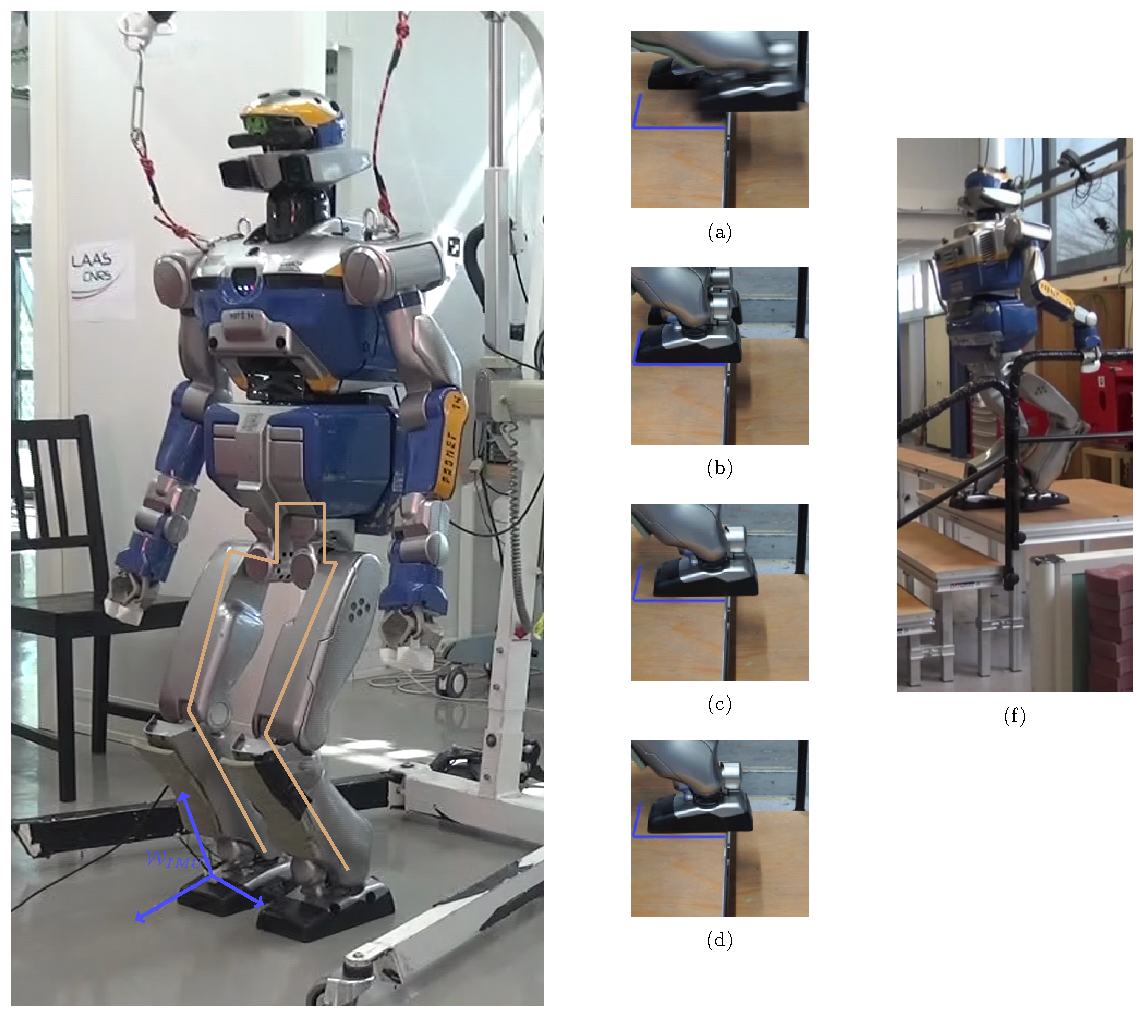
\includegraphics[width=\linewidth]{./figures/cover-figure.pdf}
% 	\caption{D(from \cite{Carpentier:ICRA:2016}).
%  }
% 	\label{fig:cover}
% \end{figure}

Graphical methods have been extensively used to implement such fusion strategies \cite{Thrun:ijrr:2006,Kaess:itro:2008} since they are well-suited to gather information from sensors
and draw conclusions. The underlying principle is to consider that desptite all the information gathered from the sensors, we still have uncertainty about the true state of the world due to sensors' imperfections.
Thus different states of the world can be considered as probable and relying probabilictic formulations is a way find out the most probable one. Furthermore, graphical representation are able to accurately model 
complex estimation problems \cite{koller2009probabilistic}. 
Fot these reasons, graphical models have been used for large modeling estimation problems by means of sparse networks of constraints and particularly in
robotics where SLAM and visual odometry problems have reached a high degree of maturity in great part thanks to these tools.
The graphical representation also allows for the design of powerful nonlinear estimation solvers, which can be built taking into account the needs for accuracy, 
robustness and CPU-performance.
In order to keep the problem tractable and maintain real-time performance a key point is to avoid the graph to be too large for a given time window.
IMUs are challenging in this regards, as their high frequency measurements create large sets of data. 
 
For this reason, \cite{LUPTON-09} proposed to pre-integrate the IMU information thus summarizing hundreds if not thousands of data into an unique
pre-integrated data over given horizon. Based on this previous work, Forster et al. \cite{forster2015imu} made efforts in making this pre-integrated data independant from the initial state it was computed on \cite{forster2015imu}.
This is particularly interessing in SLAM problems due to the possibility for this initial condition to be changed considering new available information. A standard implementation would then need to re-integrate all the data
to reconstruct the trajectory of the body, which is not necessary with \cite{forster2015imu}.
A first contribution of this paper is to reformulate the method proposed in \cite{forster2015imu} from rotation matrix to quaternion representation
and give a detailed and simpler algebraic derivation.
The second contribution is to apply this method to the estimation of foot-pose during human walking.
We will compare the level of accuracy obtained with this method against other methods classicaly used in pedestrian localization.
Finally, we describe the implementation of this pre-integration scheme in a software implementation of the graphical method designed to
allow users to easily gather information from different sensor for fusion strategies. The gathered information are then used to get a graphical model-based formulation of the problem. 
Once the formulation is completed, a non-linear least squares optimizer is used to solve the problem and find the most probable solution in the least-square sense \cite{ceres-solver}.





